\documentclass{article}

% ready for submission
\usepackage[final]{neurips_2021}
\usepackage[utf8]{inputenc} % allow utf-8 input
\usepackage[T1]{fontenc}    % use 8-bit T1 fonts
\usepackage{hyperref}       % hyperlinks
\usepackage{url}            % simple URL typesetting
\usepackage{booktabs}       % professional-quality tables
\usepackage{amsfonts}       % blackboard math symbols
\usepackage{nicefrac}       % compact symbols for 1/2, etc.
\usepackage{microtype}      % microtypography
\usepackage{xcolor}         % colors
\usepackage{algorithm2e}
\usepackage{amsmath}
\usepackage{graphicx}
\usepackage{float}
\usepackage{caption}
\usepackage{subcaption}
\usepackage{array}

\usepackage[backend=biber, style=alphabetic, sorting=ynt]{biblatex}

\addbibresource{ref.bib}

\title{CS271 Project Final Report: Sokoban Solver}

\author{
  Seokchan Ahn\\
  15288114 \\
  \texttt{seokchaa@uci.edu} \\
   \And
  Youngil Kim\\
  87561931\\
  \texttt{youngik2@uci.edu}\\
   \And
  Jinhwa Kim \\
  86727408 \\
  \texttt{jinhwak@uci.edu}
}
\begin{document}

\maketitle

\begin{abstract}
  Sokoban is a game in which the player pushes boxes around in a warehouse, trying to get them to storage locations. Since the number of possible states can grow exponentially as the board size and number of boxes increase, we suggest model-free reinforcement learning(RL) based solver for this game. Among a variety of RL algorithms, we implement Q-learning to build an efficient solver and suggest the result of our model. By tuning hyperparameters, we show an optimal result for our approach.
\end{abstract}

\section{Sokoban}
Sokoban is a game that the user pushes the boxes to the proper storage locations with a minimum number of moves. The map is consists of floor, wall, boxes, marked storage locations, and an agent which represents the user. The user can move in 4 directions: Up, Down, Left, Right, and it is not allowed to move through walls or boxes. There are two conditions for terminating the games: 1) All the boxes are on the goals. 2) Deadlocks.

\section{Q-Learning}

Q-learning is a model-free reinforcement learning algorithm to learn the value of an action in a particular state. It is an off-policy learning because the executed actions are different from the target actions that are used for learning. It updates values based on the next state's best action, but choose the action by $\epsilon$-greedy policy, which enables both exploration and exploitation.

\RestyleAlgo{ruled}
\SetKwComment{Comment}{/* }{ */}
\begin{algorithm}[H]
\caption{Q-Learning}\label{alg:one}
\KwData{State $s \in S$ , Action $a \in A(s)= \{U,D,R,L\}$}
Initialize $Q(S, A)$ as zero\;
Initialize $maxStep, \epsilon, \alpha, \gamma$\;
Initialize $s$ \Comment*[r]{initial state}
$step \gets 1$\;

\While{$step \leq maxStep$}{
  $a \gets getAction(s, \epsilon)$ \Comment*[r]{choose action using $\epsilon$-greedy policy}
  $s', r \gets getNextState(action)$ \Comment*[r]{next state, reward}
  $Q(s, a) \gets Q(s, a) + \alpha(r + \gamma \max Q(S', a) - Q(s, a))$ \Comment*[r]{update Q for s, a}
  $s \gets s'$ \Comment*[r]{update state to new state}

  \If{$isTerminal(s')$)} {
    Initialize $s$ \Comment*[r]{start over from the initial state}
  }
  $step \gets step + 1$\Comment*[r]{increase current step by 1}
}
\end{algorithm}

We use $maxStep$ as an upper-bound of the length of each episode. Though Q-learning can learn without limiting the number of steps, having an upper-bound can make the learning process more efficient by preventing exploring the states far from the goal too much. This value must be greater than the length of the episode with the optimal solution since otherwise it will never reach to the goal state. Therefore, we use $maxStep$ of $MNB$ where $M$ and $N$ denotes the board's width and height, and $B$ denotes the number of boxes, since the maximum number of steps to move one box to the storage must be less than $MN$ and there are $B$ such boxes. As a result, the time complexity of this algorithm would be $O(MNB)$ for each episode and total training time would be in proportion to the number of iterations until the Q-values converge. The space complexity would be $O((MN)^{B+1})$ because ignoring the walls, there are $MN$ positions we can place a box or a player, and there are $B$ boxes and 1 player. However, we can save the space a lot in practice by pruning branches that never able to reach a goal.

There are three hyper-parameters in Q-learning. First, $\epsilon$ decides the possibility of exploitation. In general, $\epsilon$ is initialized as a value close to 1.0, which means the agent will choose an action almost randomly, since there is no information about the expected value in the beginning. As the estimated Q-values converge, $\epsilon$ should be decayed to exploit the learned values. $\alpha$ and $\gamma$ are the learning rate and the discount factor by time for each.  

\begin{algorithm}[H]
\caption{Q-Learning Inference}\label{alg:two}
\KwData{State $s \in S$ , Action $a \in A(s)= \{U,D,R,L\}$}
Initialize $s$ \Comment*[r]{initial state}
$\epsilon \gets 0.0$ \Comment*[r]{greedy policy}

\While{$True$}{
  $a \gets getAction(s, \epsilon)$ \Comment*[r]{choose action using $\epsilon$-greedy policy}
  $s', r \gets getNextState(action)$ \Comment*[r]{next state, reward}
  $s \gets s'$ \Comment*[r]{update state to new state}
  \If{$isGoalState(s')$} {
    break \Comment*[r]{Arrived to one of the goal states}
  }
}
\end{algorithm}

In the inference time, the agent can greedy choose the best action at the current state every time. It can be done by simply using the $\epsilon$ value of zero. The time complexity would be $O(L)$ where $L$ denotes the length of the episode it generates and $L$ would be less than $M*N*B$.

\section{Implementation Details}

\subsection{States and Actions}

In the Sokoban game, states can be defined as the setting of the board. Since the positions of walls and the positions of storage are fixed, we can use the coordinations of the boxes and the player as a state. Since the order of boxes doesn't matter, we use a hash map for Q-table using $(set(boxes), player)$ as keys and Q-values as values. For actions, we use $[L, U, R, D]$ since they are all the available movements.

A Sokoban game's terminal states are 1) when all the boxes are on the storage or 2) when on a Deadlock state. In training time, we stop and re-initialize the state once the player reaches to a terminal state since we do not need to explore further. In inference time, we just stop and return the generated episode and its length.

\subsubsection{Deadlocks}

In Sokoban games, there is a state, which is called a deadlock, when an agent cannot reach any goal state, no matter what the agent moves. The only way to solve this problem is backtracking to the previous state or restarting the game. In order to solve the Sokoban game efficiently, it is inevitable to handle deadlocks properly. In our project, we handle only simple deadlocks to prune unnecessary branches in advance, but we decide not to take further actions because it is sufficient to solve Sokoban game with solely simple deadlocks detection as well as there is an overhead to detect other complicated types of deadlocks.
\footnote{http://sokobano.de/wiki/index.php?title=Deadlocks}

\paragraph{Simple deadlocks}
A simple deadlock is created by moving just one box to border lines, which makes it unable to reach any goal state, no matter what the agent moves. In the figure \ref{fig:simple}, pushing the box to a darker shaded space results in a simple deadlock.

\paragraph{Freeze deadlocks}
Freeze deadlocks refer to the situation that one of boxes becomes immovable. If a box becomes immovable while not being located on a goal, the game is deadlocked. In the figure \ref{fig:freeze}, pushing the box one square up results in a freeze deadlock.

\paragraph{Corral deadlocks}
Corral indicates a zone that the agent cannot access. Corral deadlocks can be created when deadlock happens if the agent is not able to move the box because of presence of corral. In the figure \ref{fig:corral}, marked area with little blue quadrats is a corral, and it is not reachable for the agent. Pushing the lower box to the right square results in a corral deadlock.

\begin{figure}
     \centering
     \begin{subfigure}[b]{0.3\textwidth}
         \centering
         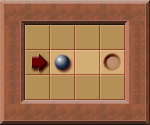
\includegraphics[width=\textwidth]{SimpleDeadlockExample.png}
         \caption{Simple Deadlock}
         \label{fig:simple}
     \end{subfigure}
     \hfill
     \begin{subfigure}[b]{0.3\textwidth}
         \centering
         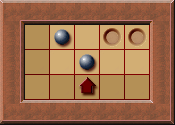
\includegraphics[width=\textwidth]{FreezeDeadlockExample.png}
         \caption{Freeze Deadlock}
         \label{fig:freeze}
     \end{subfigure}
     \hfill
     \begin{subfigure}[b]{0.3\textwidth}
         \centering
         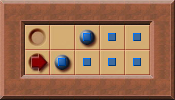
\includegraphics[width=\textwidth]{CorralDeadlockExample.png}
         \caption{Corral Deadlock}
         \label{fig:corral}
     \end{subfigure}
        \caption{Three simple graphs}
        \label{fig:deadlocks}
\end{figure}

\subsection{Rewards}
Rewards are the most important part in reinforcement learning since it decides which actions are good or bad and how good or bad they are. We defined the categories of rewards as below.

% Please add the following required packages to your document preamble:

\begin{table}[H]
\centering
\resizebox{\textwidth}{!}{%
\begin{tabular}{|l|l|p{8cm}|}
\hline
Category          & Reward & Description                                                                                                                         \\ \hline
MOVE              & -0.1   & To prevent looping infinitely, give small penalty for each move                                                                     \\ \hline
BOX\_ON\_STORAGE &
  1.0 &
  Since it may takes too many steps to the final goal, updating Q-values from the final reward is difficult. Therefore, giving rewards for achieving intermediate goals can make the Q converge faster. \\ \hline
BOX\_OFF\_STORAGE & -1.0   & Give penalty for pushing a box away from a storage.                                                                                 \\ \hline
ALL\_ON\_STORAGE  & 10.0   & Give reward when the player successfully finishes the game.                                                                         \\ \hline
DEADLOCK          & -10.0  & Once it gets to a deadlock state, it can never be solved afterwards. Therefore, give a great penalty and initialize the state again. \\ \hline
MOVE\_TO\_WALL    & -1.0   & Trying to go toward a wall or a box in front of another box or a wall is not worth. Therefore, give a small penalty.                \\ \hline
\end{tabular}%
}
\caption{Categories of rewards and their values}
\label{tab:rewards}
\end{table}

\section{Experiments}
\subsection{Hyperparameter Optimization}
A hyperparameter is a parameter whose value is used to control the learning process. These parameters are tunable and they could directly affect to the model performance. Thus, optimizing those parameters is inevitable to maximize the performance. We explore the hyperparmeter space by grid search to figure out the optimal hyperparameters. 

\paragraph{Learning rate $\alpha$}
The learning rate is used to determine to what extent newly acquired information overrides old information. When the learning rate is set to 0, the agent learn nothing. In case of 1, update current Q-value by the amount of TD-error. We experiment tuning the learning rate from 0 to 1 in increments of 0.2 for each step.

\paragraph{Discount factor $\gamma$} The discount factor is used to determine the importance of future rewards. If the discount factor is set to 0, do not consider the next Q-value at all and with the discount factor of 1, fully attend the next step's Q-value. We experiment tuning the discount factor from 0 to 1 in increments of 0.2 for each step.

\paragraph{$\epsilon$-decay rate} The $\epsilon$-decay rate decides how much to reduce the $\epsilon$ for every successful episode. We need to decide $\epsilon$-decay rate between 0 and 1 because we need to increase the possibility of exploitation over exploration as learn more by decreasing $\epsilon$. We experiment varying $\epsilon$-decay rate from 0.5 to 0.9 in increments of 0.1 for each step. Initially, we set $\epsilon$ as 0.9, and it is adjusted with the $\epsilon$-decay rate during the iteration.

Since we use $\epsilon$-greedy method, which is a stochastic component, the policy can be varied for each training even with the same hyperparameters. Thus, We iterate training 5 times and choose the best hyperparameters based on the mean of the results.

To discover the optimal hyperparameters, we evaluate the learned Q-values by three criteria. First, we check whether the Q-learning is converged. We define convergence as the greedy policy stalls for 5 consecutive evaluations during the training process. To expedite experiments, when the number of iteration exceeds a specific number, 100,000, we consider it as diverging and stop learning. Second, we compare the length of the episode when following the greedy policy. We prioritize the Q that generates shorter episode. Finally, we prefer the parameter that converges in shorter number of updates.

In the experiment, we use the input data provided by the class, $sokoban01.txt$, because $sokoban00.txt$ is too trivial to measure performance of the algorithm.

\section{Results}

\begin{table}[H]
\centering
\resizebox{\textwidth}{!}{
%
\begin{tabular}{| c|c|c||c||c||c |}
\hline
Learning rate $\alpha$ & Discount factor $\gamma$ & $\epsilon$-decay rate & Converged? & length of episode & \# of steps                                         \\ \hline
0.2 & 0.2 & 0.5 & No & - & -                                      \\ \hline
0.2 & 0.2 & 0.7 & No & - & -                                      \\ \hline
0.2 & 0.2 & 0.9 & No & - & -                                      \\ \hline
0.2 & 1.0 & 0.5 & Yes & 22 & 74,400                                      \\ \hline
0.2 & 1.0 & 0.7 & Yes & 22 & 51,620                                      \\ \hline
0.2 & 1.0 & 0.9 & Yes & 22 & 62,100                                      \\ \hline
0.6 & 0.6 & 0.5 & Yes & 36 & 39,440                                      \\ \hline
0.6 & 0.6 & 0.7 & Yes & 36 & 42,480                                      \\ \hline
0.6 & 0.6 & 0.9 & Yes & 36 & 62,450                                      \\ \hline
1.0 & 0.2 & 0.5 & Yes & 36 & 36,020                                      \\ \hline
1.0 & 0.2 & 0.7 & Yes & 36 & 49,820                                      \\ \hline
1.0 & 0.2 & 0.9 & Yes & 36 & 42,760                                      \\ \hline
1.0 & 1.0 & 0.5 & Yes & 22 & 25,960                                      \\ \hline
1.0 & 1.0 & 0.7 & Yes & 22 & 23,740                                      \\ \hline
1.0 & 1.0 & 0.9 & Yes & 22 & 29,800                                      \\ \hline

\end{tabular}%
}
\caption{Parameter Tuning Results}
\label{tab:tuning}
\end{table}

Table \ref{tab:tuning}, shows a partial results of hyperparameter exploration. We have found that the algorithm does not work when both the learning rate $\alpha$ and the discount factor $\gamma$ are low, regardless of the $\epsilon$-decay rate. Also, surprisingly, the algorithm tends to find a non-optimal episode when either the learning rate $\alpha$ or the discount factor $\gamma$ is high.

The Q-learning converged to the optimal policy the fastest after 23,740 iterations, with the learning rate $\alpha$ of \textbf{1.0}, the discount factor $\gamma$ of \textbf{1.0}, and the $\epsilon$-decay rate of \textbf{0.7}.

\begin{figure}[h]
    \centering
    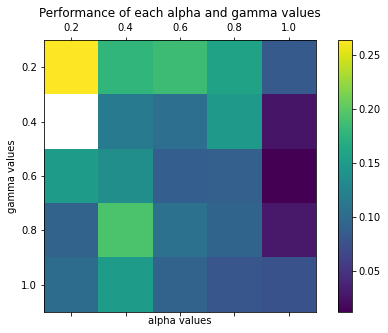
\includegraphics[width=10cm]{output.png}
    \caption{Performance on each learning rate $\alpha$ and discount factor $\gamma$}
    \label{fig:output}
\end{figure}

\paragraph{Comparison of performance for two hyperparameters}
To find the relationship between hyper-parameter setting and performance, we plot each result in the respect of two hyper parameter values: $\alpha$ and $\gamma$. We consider two factors, \textit{length of episode} and \textit{number of steps}, as the performance of the model and normalize each of the values and calculate the weighted sum of the two values. Since the length of episode is a more important factor, we give 0.8 as a weight for the length of the episode and 0.2 for the number of steps. Figure \ref{fig:output} shows the result of performance and the darker square means more optimal result and white square means not converged case. The result shows that higher $\alpha$ tends to make a better result regardless of the value of $\gamma$.


\section{Conclusion}
In this project, we defined the states, actions, and rewards of the Sokoban game to bring the it to the reinforcement learning problem, and implemented a Sokoban solver using the Q-learning algorithm. To optimize the Q-learning, we explored the hyperparameter space using grid search. And we averaged the results after running 5 times for each hyperparameter set, since it contains the $\epsilon$-greedy method, which is a stochastic component. As a result, we found the optimal hyperparemeter, the learning rate $\alpha$ of \textbf{1.0}, the discount factor $\gamma$ of \textbf{1.0}, and the $\epsilon$-decay rate of \textbf{0.7}, for the $sokoban01.txt$ problem. With that settings, the length of the episode to the goal state was 22 and it took 23,740 iterations to be converged in average.

% \appendix

% \section{Appendix}

% Optionally include extra information (complete proofs, additional experiments and plots) in the appendix.
% This section will often be part of the supplemental material.

% \printbibliography

\section{References}

[1] Russell, S. J., Norvig, P., \& Davis, E. (2010). Artificial intelligence: a modern approach. 4th ed. Upper Saddle River, NJ: Prentice Hall.

% [2] Ketan Doshi. (2020). Reinforcement Learning Explained Visually (Part 4): Q Learning, step-by-step. Towards Data Science. https://towardsdatascience.com/reinforcement-learning-explained-visually-part-4-q-learning-step-by-step-b65efb731d3e

\end{document}